\documentclass[12pt]{article}
\pagestyle{empty}
\usepackage[utf8]{inputenc}
\usepackage[T2A]{fontenc}
\usepackage[english,russian]{babel} 
\usepackage{cmap}
\usepackage{amsthm}
\usepackage{amsmath}
\usepackage{amssymb}
\usepackage{tikz}
\usepackage{listings}
\textheight=24cm
\textwidth=16cm
\oddsidemargin=0pt
\topmargin=-1.5cm
\parindent=24pt
\parskip=0pt
\tolerance=2000
\flushbottom 

\begin{document}
\pagestyle{plain}
\begin{titlepage}
\title{Многорукие бандиты}
\author{Селиханович Даниил, МФТИ ФУПМ, 572 группа}
\maketitle
\thispagestyle{empty}

		\begin{center}
			\begin{Large}
				Постановка задачи
			\end{Large}
		\end{center}
\textbf{Многорукие бандиты}. Имеется два «одноруких бандита» (так называют игровые автоматы с ручкой, дергая за которую получаем случайный выигрыш). Вероятность выиграть 1 франк на первом автомате $p_1 > 0$ (с вероятностью $1 - p_1$ выигрыш равен 0), а на втором — $p_2 > 0$. Обе вероятности неизвестны. Игрок может в любом порядке раз дергать за ручки «одноруких бандитов». Стратегией игрока является выбор ручки на каждом шаге, в зависимости от результатов всех предыдущих шагов, так чтобы суммарный выигрыш был бы максимальным. Приведите стратегию игрока. Предложите свое обобщение задачи.
\end{titlepage}
\newpage
\tableofcontents


\newpage
\section{Динамическое программирование.}
\subsection{Испытания Бернулли.}
Постановка задачи: у нас имеется последовательность подбрасываний монетки, о <<честности>> которой нам ничего не известно. Требуется определить, какова вероятность получить орёл или решку в следующем подбрасывании.
\newline
\newline
Обозначим вероятность выпадения орла через $q$, случайные величины, соответствующие $i$-му подбрасыванию монетки, через $X_i$, а их значения через $x_i$: $x_i = 1$, если выпал орёл и $x_i = 0$ для решки. По формуле Байеса плотность вероятности $f\left(q\right) = \Prob \Bigl (q\; \Bigl|\; X_1 = x_1, \dots, X_n = x_n \Bigr )$ вычисляется так:
\begin{align}
\Prob \Bigl (q\; \Bigl|\; X_1 = x_1, \dots, X_n = x_n \Bigr ) = \frac{\Prob(q)\Prob \Bigl (X_1 = x_1, \dots, X_n = x_n \; \Bigl|\; q \Bigr )}{\Prob \Bigl (X_1 = x_1, \dots, X_n = x_n \Bigr )}. 
 \end{align}
Мы будем считать, что априорное распределение <<честности>> монетки \underline{\textbf{равномерное}}, то есть пока мы не видели ни одного результата, мы вообще ничего не можем сказать о вероятности выпадения орла и считаем все такие вероятности одинаково возможными: $\Prob(q) = 1$ при $0 \leq q \leq 1$ и $\Prob(q) = 0$ иначе. 
\begin{align}
\Prob \Bigl (X_1 = x_1, \dots, X_n = x_n \; \Bigl|\; q \Bigr ) = \prod\limits_{i = 1}^{n} q^{x_i}(1 - q)^{1 - x_i} = q^s(1 - q)^{n - s}.
\end{align} Здесь $s$ - число выпадений орлов в эксперименте из $n$ подбрасываний.
\newline
\newline
Дискретная формула полной вероятности в непрерывном случае, как в данной задаче, пример вид:
\begin{multline*}
\Prob \Bigl (X_1 = x_1, \dots, X_n = x_n\Bigr ) = \int \limits_0^1 q^s(1 - q)^{n - s} dq = 
B(s + 1, n - s + 1) = \\ \frac{\Gamma(s + 1) \Gamma(n - s + 1)}{\Gamma(n + 2)} = \frac{s! (n - s)!}{(n + 1)!}
\end{multline*}
Получили, что 
\begin{align}
\Prob \Bigl (q\; \Bigl|\; X_1 = x_1, \dots, X_n = x_n \Bigr ) = \frac{(n + 1)!}{s! (n - s)!}q^s(1 - q)^{n - s}
\end{align}
Вычислим матожидание $\mathsf E[q]$ выпадения орла в следующем подбрасывании монетки при условиях эксперимента $X_1 = x_1, \dots, X_n = x_n$:
\begin{multline*}
\mathsf E [q] = \int \limits_0^1 qf(q)\, dq = \int \limits_0^1 q \frac{(n + 1)!}{s! (n - s)!}q^s(1 - q)^{n - s}\, dq = \frac{(n + 1)!}{s! (n - s)!}  \int \limits_0^1 q^{s + 1}(1 - q)^{n - s}\, dq = \\ = \frac{(n + 1)!}{s! (n - s)!} B(s + 2, n - s + 1) =  \frac{(n + 1)!}{s! (n - s)!} \frac{\Gamma(s + 2) \Gamma(n - s + 1)}{\Gamma(n + 3)} = \\ = \frac{(n + 1)!}{s! (n - s)!} \frac{(s+ 1)! (n - s)!}{(n + 2)!} = \frac{s + 1}{n + 2}.$ $\textbf{(4)}
\end{multline*}
\newpage
\subsection{Алгоритм поиска ожидаемой максимальной прибыли.}
Пусть мы имеем $k$ разных <<одноруких бандитов>>. Будем обозначать состояние игрока после $n_1$ использований 1-ой ручки, из которых только $w_1$ были успешными, $\dots, n_k$ использований $k$-ой ручки, из которых только $w_k$ были успешными, через $S = \Bigl\{(n_1, w_1), \dots, (n_k, w_k)\Bigr\}$, а $V^*(S)$ через ожидаемый максимальный выигрыш для состояния с данной историей, если всего можно делать $h$ выборов.
\newline
\newline
Тогда задача сводится к вычислению $V^*\Bigl((0, 0), \dots, (0, 0)\Bigr)$ для данного числа выборов $h$. Базой рекурсии, которую мы хотим составить, будет служить очевидное равенство:
$$V^*\Bigl(n_1, w_1), \dots, (n_k, w_k)\Bigr) =  0 \text{ для всех таких }n_1, \dots, n_k: \sum \limits_{i = 1}^{k} n_i = h \eqno(5)$$. 
Если обозначить через $\rho_i$ ожидаемую вероятность того, что после истории испытаний на ручке $i$ $(n_i, w_i)$ игрок в состоянии $S$ получит выигрыш после выбора ручки $i$, то можем выписать следующую рекурренту:
\begin{multline*} \textbf{(6)}$ $V^*\Bigl((n_1, w_1), \dots, (n_k, w_k)\Bigr) = \\ = \max_{1 \leq i \leq k} \Bigl(\rho_i \Bigl\{1 + V^*\Bigl((n_1, w_1), \dots, (n_i + 1, w_i + 1), \dots\Bigr) \Bigr\} + (1 - \rho_i)V^*\Bigl((n_1, w_1), \dots, (n_i + 1, w_i), \dots\Bigr)\Bigr)
\end{multline*}
Согласно \textbf{(4)} можем считать, что $\rho_i = \frac{w_i + 1}{n_i + 2}$ в соответствии с условием задачи, так как вероятности выигрыша $p_i$ могут быть произвольными ненулевыми. 
\newline
\newline
Замечаем, что данная рекуррента с учётом начальных условий позволяет определить $V^*\Bigl((0, 0), \dots, (0, 0)\Bigr)$ для данного числа выборов $h$, не проводя сам эксперимент. Тем самым возникает наивный алгоритм действий игрока, желающего получить ожидаемый максимальный выигрыш при игре с однорукими бандитами.
\newpage
\begin{center}
	\begin{Large}
			Алгоритм
	\end{Large}
\end{center}
1) предрасчётом вычислить таблицу $V^*\Bigl((n_1, w_1), \dots, (n_k, w_k)\Bigr)$ для всех $n_1, \dots, n_k, w_1, \dots, w_k: 0 \leq w_i \leq n_i, \sum \limits_{i = 1}^{k} n_i \leq h$. Сложность заполнения таблицы - $O(k|V^*|)$, где $|V^*| = O\Bigl((h + 1)^k \sum \limits_{i = 0}^{h} {i + k - 1 \choose i}\Bigr) = O\Bigl(h^k {\binom{h + k}{k}}\Bigr)$ - размер заполняемой+- таблицы. В общем случае получаем экспоненциальное время заполнения от $h$, но при небольшом числе ручек $k$ получаем полином от $h$ - так, для двух ручек получим сложность заполнения таблицы $O(h^4)$.
\newline
\newline
2) на каждом шаге с данным фиксированным состояние опыта 
$S = \Bigl\{(n_1, w_1), \dots, (n_k, w_k)\Bigr \}$ выбирать действие $i$, для которого достигается
$$ \max_{1 \leq i \leq k} \Bigl(\rho_i \Bigl\{1 + V^*((n_1, w_1), \dots, (n_i + 1, w_i + 1), \dots) \Bigr\} + (1 - \rho_i)V^*((n_1, w_1), \dots, (n_i + 1, w_i), \dots)\Bigr).$$
3) переходить в новое состояние $S_{new}$.
\newline
\newline
\underline{\textbf{Анализ алгоритма}}: при значениях $k$, сравнимых с $h$, время заполнения экспоненциально от времени игры, так что можем использоваться только в тех случаях, когда нужно планировать игру не слишком далеко. По сути - полный перебор всех возможных событий. Зато таблица $V^*\Bigl((n_1, w_1), \dots, (n_k, w_k)\Bigr)$ может использоваться многократно.
\begin{figure}
  \begin{center}
  	\caption{Порядок заполнения таблицы}
    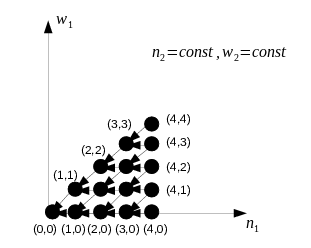
\includegraphics{short_last.png}
  \end{center}
\end{figure}
\begin{figure}
  \begin{center}
  	\caption{Несимметричные вероятности}
    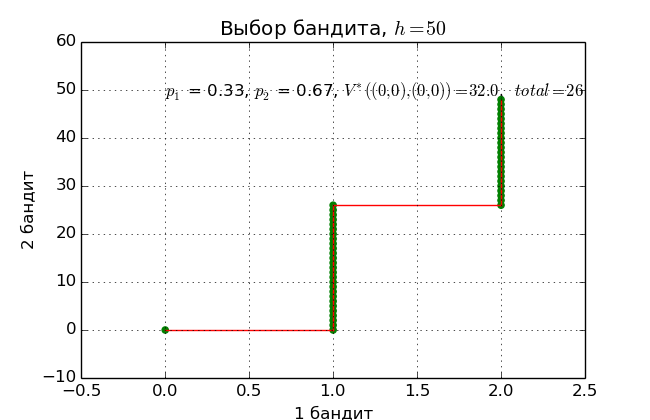
\includegraphics{2bandits-pic1.png}
  \end{center}
\end{figure}
\begin{figure}
  \begin{center}
  	\caption{Несимметричные вероятности}
    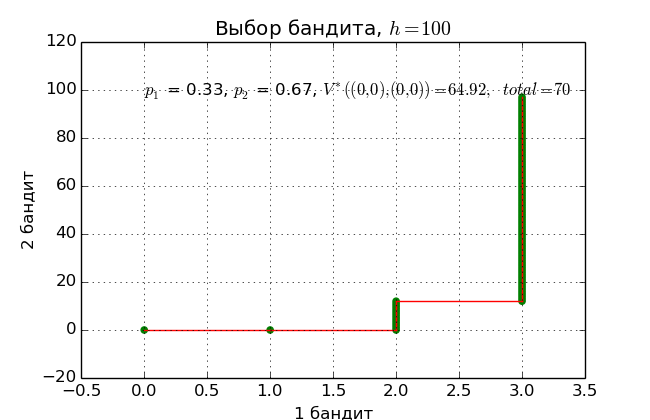
\includegraphics{2bandits-pic2.png}
  \end{center}
\end{figure}
\begin{figure}
  \begin{center}
  	\caption{Несимметричные вероятности}
    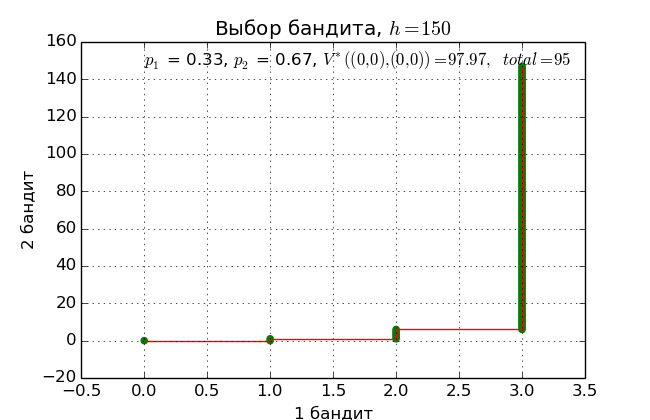
\includegraphics{2bandits-pic3.png}
  \end{center}
\end{figure}
\begin{figure}
  \begin{center}
  	\caption{Несимметричные вероятности}
    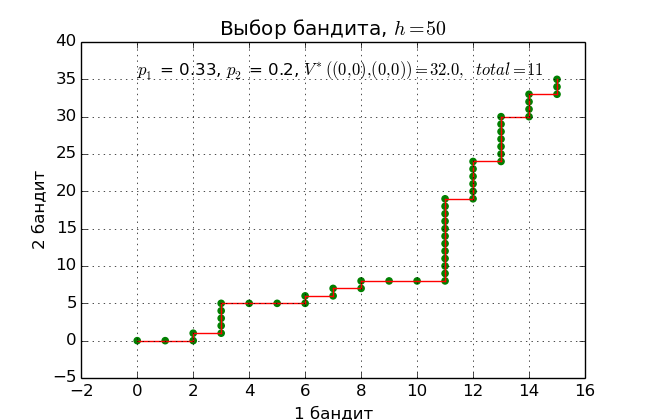
\includegraphics{2bandits-pic4.png}
  \end{center}
\end{figure}
\begin{figure}
  \begin{center}
  	\caption{Несимметричные вероятности}
    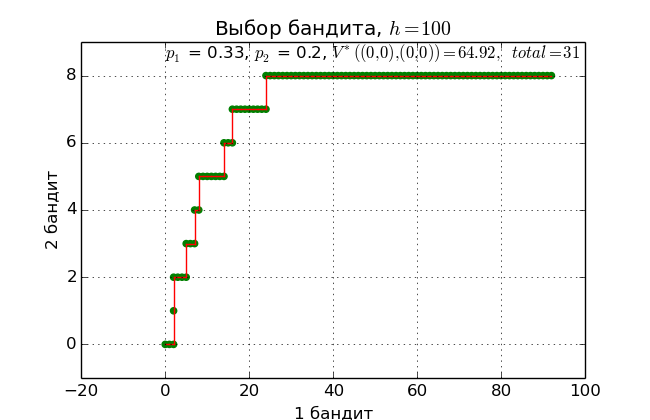
\includegraphics{2bandits-pic5.png}
  \end{center}
\end{figure}
\begin{figure}
  \begin{center}
  	\caption{Несимметричные вероятности}
    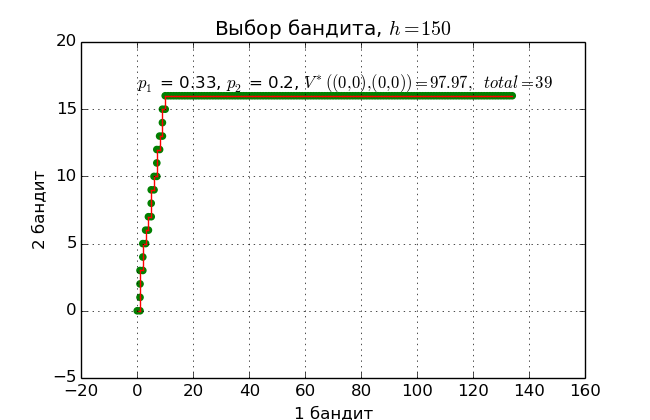
\includegraphics{2bandits-pic6.png}
  \end{center}
\end{figure}
\begin{figure}
  \begin{center}
  	\caption{Симметричные вероятности}
    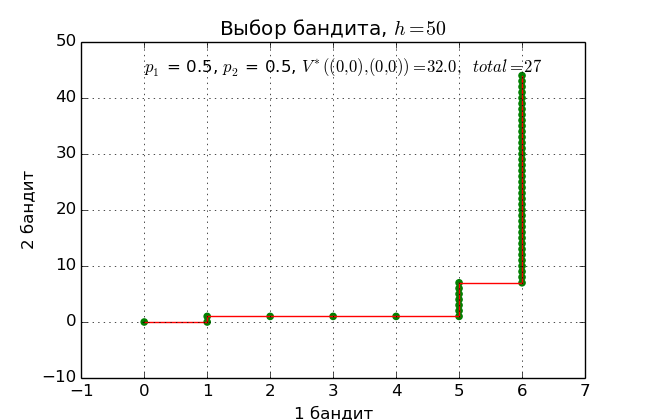
\includegraphics{2bandits-pic7.png}
  \end{center}
\end{figure}
\begin{figure}
  \begin{center}
  	\caption{Симметричные вероятности}
    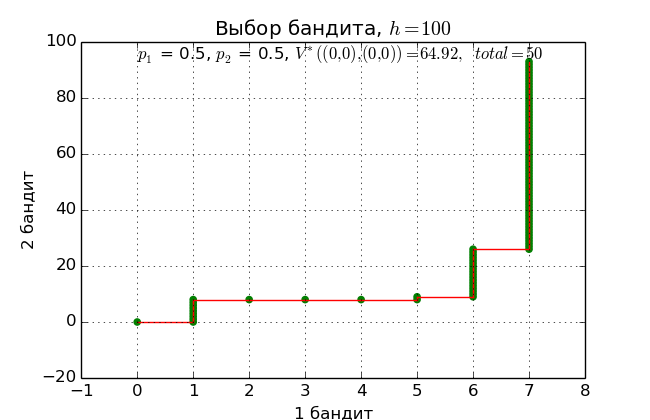
\includegraphics{2bandits-pic8.png}
  \end{center}
\end{figure}
\begin{figure}
  \begin{center}
  	\caption{Симметричные вероятности}
    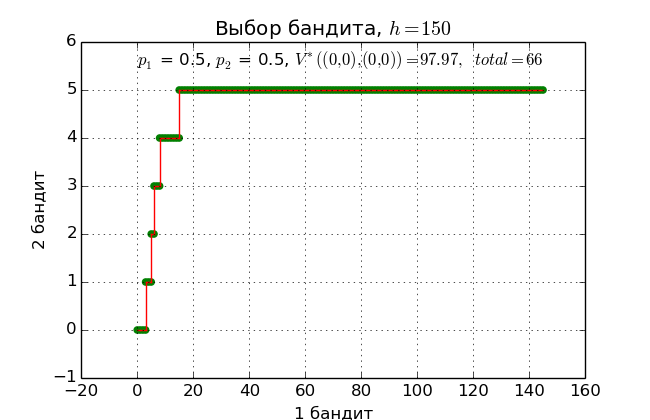
\includegraphics{2bandits-pic9.png}
  \end{center}
\end{figure}
\newpage
\section{Заключение}
Выражаю благодарность \underline{\textbf{Гасникову Александру Владимировичу}} 
\newline
 и \underline{\textbf{Сувориковой Александре}} за помощь в исследовании задачи.
\begin{thebibliography}{10}
\bibitem{1} 
\textit{Баяндина А. С., Гасников А.В., Гулиев Ф.Ш., Лагуновская А.А.} 
Безградиентные двухточечные методы решения задач стохастической 
негладкой выпуклой оптимизации при наличии малых шумов не случайной природы: https://arxiv.org/ftp/arxiv/papers/1701/1701.03821.pdf.
\bibitem{2}  \textit{Гасников А. В., Нестеров Ю.Е., Спокойный В.Г.} 
Об эффективности одного метода рандомизации зеркального спуска в задачах онлайн оптимизации:
https://arxiv.org/pdf/1410.3118.pdf.
\bibitem{3}  \textit{Гасников А. В., Крымова Е.А., Лагуновская А.А., Усманова И.Н., Федоренко Ф.А.} 
Стохастическая онлайн оптимизация. 
Одноточечные и двухточечные нелинейные многорукие 
бандиты. Выпуклый и сильно выпуклый случаи:
https://arxiv.org/ftp/arxiv/papers/1509/1509.01679.pdf.
\bibitem{4}  \textit{Гасников А. В., Крымова Е.А., Лагуновская А.А., Усманова И.Н., Федоренко Ф.А.} 
Безградиентные прокc-методы с неточным оракулом для негладких задач выпуклой стохастической оптимизации на симплексе:
https://arxiv.org/ftp/arxiv/papers/1412/1412.3890.pdf.
\bibitem{5}  \textit{Аникин А. С., Гасников А.В., Двуреченский П.Е., Тюрин А.И., Чернов А.В.} 
Двойственные подходы к задачам минимизации сильно выпуклых функционалов простой структуры при аффинных ограничениях:
https://arxiv.org/ftp/arxiv/papers/1602/1602.01686.pdf.
\bibitem{6} Лекция Зорича В.А про концентрацию меры:
\newline $http://www.mathnet.ru/php/seminars.phtml?option_lang=rus\&presentid=14604$.
\bibitem{7} \textit{Николенко C. И., Тулупьев А.Л.} 
Самообучающиеся системы. Российская академия наук. Санкт-Петербургский институт информатики и автоматизации РАН. Москва, Издательство МЦНМО, 2009.
\bibitem{8}
\textit{Bubeck S., Cesa-Bianchi N.} Regret analysis of stochastic and nonstochastic multi-armed bandit problems, Foundation and Trends in Machine Learning, 5:1 (2012) 1–122; Lugosi G., Cesa-Bianchi N. Prediction, learning and games. New York: Cambridge University Press, 2006.
\bibitem{9}
\textit{Lev Bogolubsky, Pavel Dvurechensky, Alexander Gasnikov, Gleb Gusev, Yurii Nesterov, Andrey Raigorodskii, Aleksey Tikhonov, Maksim Zhukovskii} 
Learning Supervised PageRank with Gradient-Free
Optimization Methods:
https://arxiv.org/pdf/1411.4282.pdf.
\end{thebibliography}
\begin{center}
	\begin{Large}
			Спасибо за внимание!
	\end{Large}
\end{center}
\newpage
\section{Дополнение. Метод зеркального спуска в задачах стохастической выпуклой оптимизации.}
\subsection{Постановка задачи в терминах оптимизации.}
Рассмотрим смежную задачу о нелинейных бандитах с шумом, в которой выбор ручки приносит нам случайные потери на шаге $k$ ручки $i(k) \; (1 \leq i \leq n)$, равные $f_{i(k)}^k$, зависящие от номера шага, номера ручки и от того, какой стратегии мы придерживались до шага $k$ включительно. Наша стратегия на шаге $k$ описывается вектором распределения вероятностей $x^k \in S_n(1) = \{x \geq 0 \;|\; \sum \limits_{i = 1}^{n} x_i = 1\}$, согласно которому мы независимо ни от чего выбираем ручку, которую будем дёргать. Все, чем мы располагаем на шаге $k$, это вектором 
$$
\Bigl((x^1, i(1), f_{i(1)}^1); \dots; (x^{k - 1}, i(k - 1), f_{i(k - 1)}^{k - 1})\Bigr).
$$
Мы считаем, что потери на $k$-ом шаге $f^k$ зависят от $x^k$ (но не от результата разыгрывания из распределения $x^k$), зависят от $(x^1, \dots, x^{k -1})$ и от результатов соответствующих разыгрываний, а также зависят от $(f^1, \dots, f^{k - 1})$. Таким образом, целью является организовать процедуру выбора ручек, чтобы ожидаемые суммарные потери были бы минимальны.
\newline
\newline
Предполагаем, что функция $f(x^k)$ выпуклая на $Q = S_n(1)$  и равна потерям после выбора на $k$-ом шаге вектора вероятностей $x^k$. Однако игрок не может наблюдать значение самой функции $f(x)$, а видит лишь зашумленную реализацию значений этой функции:
$$
\widetilde f(x^k, \xi^k) = f(x^k, \xi^k) + \delta(x^k, \xi^k), \eqno(7)
$$
$$
\mathsf E_{\xi^k}(f(x^k, \xi^k)) = f(x^k), |\delta(x^k, \xi^k)| < \delta. \eqno(8)
$$
Предполагается, что $\{\xi^k\}_k$ - независимые одинаково распределённые случайные величины (их реализации одинаковы для всех игроков), функция $f(x, \xi)$ как функция $x$ в $\mu_0$-окрестности выпуклого множества $Q$ является:
\begin{itemize}
\item \textbf{(9)} выпуклой;
\item удовлетворяющей условию \textbf{(10)} $|f(x, \xi) - f(y, \xi)| \leq M \bigl\| y - x \bigr\|_2\; \forall x,y,\xi.$
\end{itemize}
Успешность стратегии игрока, сыгравшего $N >> 1$ раз, характеризуется величиной:
$$
Regret_f\Bigl(\{x^k\}_{k = 0}^{N - 1}\Bigr) = \mathsf E \Bigl\{\frac{1}{N}\sum \limits_{k = 0}^{N - 1}f(x^k) \Bigr\} - \min_{x \in Q} f(x)\eqno(11)
$$
Пусть $x^k = x_*$ - оптимальная стратегия игрока и игрок начинает в состоянии $x^0$. Введём прокс-функцию $d(x) \geq 0$ $(d(x^0) = 0)$, которая предполагается сильно выпуклой относительно евклидовой нормы, и определим $R^2 = V(x_*, x^0)$, где прокс-расстояние (расстояние Брэгмана) определяется формулой: 
$$
V(x, z) = d(x) - d(z) - \langle \nabla d(z), x - z \rangle. \eqno(12)
$$
На каждой итерации можно один раз обратиться к оракулу за зашумленным значением стохастического градиента $\nabla_x \widetilde f(x^k, \eta^k)$.
Пусть для любых $\widetilde N \leq N$ выполнено ($\Theta^{k - 1}$ - сигма алгебра, порождённая случайными величинами $\eta^1, \dots, \eta^{k - 1}$):
 $$\sup \limits_{ \{x^k = x^k(\xi^1, \dots, \xi^{k - 1})\}_{k = 1}^{\widetilde N} \in Q} \mathsf E \Bigl\{\frac{1}{\widetilde N} \sum \limits_{k = 1}^{\widetilde N} \Bigl \langle \mathsf E_{\eta^k} \Bigl \{\nabla_x f(x^k, \eta^k) - \nabla_x \widetilde f(x^k, \eta^k)\;|\; \Theta^{k - 1}\Bigr \}, x^k - x_* \Bigr \rangle \Bigr\}\leq \sigma; \eqno(13)$$
 $$
 \mathsf E_{\eta^k} \Bigl\{\nabla_x f(x^k, \eta^k) \Bigr\} = \nabla f(x^k), \mathsf E_{\eta^k} \Bigl\{\bigl\| \nabla_x \widetilde f(x^k, \eta^k)\bigr\|_2^2 \Bigr\} \leq {\widetilde M}^2, \eqno(14)
 $$
 где $\{\eta^k\}_{k = 0}^{N - 1}$ - независимые одинаково распределённые случайные величины.
\subsection{Оценка регрета.}
 Метод зеркального спуска состоит в выборе на очередном шаге: 
 $$
 \textbf{(15)}\; x^{k + 1} = Mirr_{x^k} \Bigl(h \nabla_x \widetilde f(x^k, \eta^k) \Bigr), Mirr_{x^k} (v) = \arg \min_{x \in Q} \Bigl\{ \Bigl \langle v, x - x^k \Bigr \rangle + V(x, x^k) \Bigr\},
 $$
 где шаг спуска $h$ будет впоследствии выбран.
 \newline
 \newline
 Основное свойство МЗС:
 \newline
 \newline
 $\textbf{(16)}$ $2V(x, x^{k + 1}) \leq 2V(x, x^k) + 2h \Bigl \langle \nabla_x \widetilde f(x^k, \eta^k), x - x^k \Bigr \rangle + h^2 \Bigl\| \nabla_x \widetilde f(x^k, \eta^k)\Bigr\|_2^2.
 $
 Тогда можем получить: 
$$
 \textbf{(17)} \; f(x^k) - f(x) \leq_{\textbf{(9)}} \Bigl \langle \nabla f(x^k), x^k - x \Bigr \rangle =_{\textbf{(14)}} \Bigl \langle \mathsf E_{\eta^k} \Bigl\{\nabla_x f(x^k, \eta^k)\; |\; \Theta^{k - 1} \Bigr\}, x^k - x \Bigr \rangle \leq_{\textbf{(8)}}
 $$ 
 \begin{multline*}
 \leq \Bigl \langle \mathsf E_{\eta^k} \Bigl\{\nabla_x f(x^k, \eta^k)\; |\; \Theta^{k - 1}\Bigr\} - \nabla_x \widetilde f(x^k, \eta^k) , x^k - x \Bigr \rangle + \frac{1}{h}\Bigl(V(x, x^k) - V(x, x^{k + 1})\Bigr) + \frac{h}{2}\bigl\| \nabla_x \widetilde f(x^k, \eta^k)\bigr\|_2^2. 
 \end{multline*}
 Берём условное матожидание $E_{\eta^k} \Bigl\{\cdot \; |\; \Theta^{k - 1} \Bigr\}$ от обеих частей неравенства $ \textbf{(17)}$ и воспользуемся неравенством $(14)$:
  \begin{multline*}
 \textbf{(18)} \; f(x^k) - f(x) \leq \Bigl \langle \mathsf E_{\eta^k} \Bigl\{\nabla_x f(x^k, \eta^k) - \nabla_x \widetilde f(x^k, \eta^k) \; |\; \Theta^{k - 1} \Bigr\} , x^k - x \Bigr \rangle + \\ + \frac{1}{h}\Bigl(V(x, x^k) - E_{\eta^k} \Bigl\{V(x, x^{k + 1}) \; |\; \Theta^{k - 1} \Bigr\}\Bigr) + \frac{h}{2}{\widetilde M}^2.
 \end{multline*}
 Суммируем последнее неравенство по $k = 0, \dots, N - 1$, делим на $N$ обе части, а затем берём полное математическое ожидание от обеих частей и полагаем $x = x_* = \min_{x \in Q} f(x)$ и если такое $x^*$ не единственно, тогда выбираем то, которое доставляет минимум $R^2 = V^*(x_*, x^0)$:
\begin{multline*}
 \textbf{(19)} \; \mathsf E \Bigl\{\frac{1}{N}\sum \limits_{k = 0}^{N - 1}f(x^k) \Bigr\} - f(x_*)  \leq  \mathsf E \Bigl\{\frac{1}{N} \sum \limits_{k = 0}^{N - 1} \Bigl \langle \mathsf E_{\eta^k} \Bigl \{\nabla_x f(x^k, \eta^k) - \nabla_x \widetilde f(x^k, \eta^k)\;|\; \Theta^{k - 1}\Bigr \}, x^k - x_* \Bigr \rangle \Bigr\} + \\ + \frac{1}{hN}\Bigl(V(x_*, x^0) - V(x_*, x^{N})\Bigr) +  \frac{h}{2}{\widetilde M}^2.
\end{multline*}
В силу того, что расстояние Брэгмана всегда неотрицательно, то с учётом (13) получаем оценку на регрет в зависимости от шага $h$ в МЗС:
$$
Regret_f\Bigl(\{x^k\}_{k = 0}^{N - 1}\Bigr) \leq \sigma + \frac{R^2}{hN} + \frac{h}{2}{\widetilde M}^2. \eqno(20)
$$
Здесь $R^2 = V(x_*, x^0)$. Желаем минимизировать оценку по $h$, значит выбираем 
$$
h = \sqrt{\frac{2R^2}{N{\widetilde M}^2}} \eqno(21)
$$
При такой оценке получаем 
$$
Regret_f\Bigl(\{x^k\}_{k = 0}^{N - 1}\Bigr) \leq \sigma + \sqrt{\frac{2R^2{\widetilde M}^2}{N}} \eqno(22)
$$
Значит, после 
$$
N = \frac{2R^2{\widetilde M}^2}{\varepsilon^2} \eqno(23)
$$
испытаний мы получим оценку
$$
Regret_f\Bigl(\{x^k\}_{k = 0}^{N - 1}\Bigr) \leq \sigma + \varepsilon. \eqno(24)
$$
\subsection{Сглаживание задачи.}
Пусть $\widetilde e \in RB_2^n(1)$ - случайный вектор, равномерно распределённый на шаре единичного радиуса в норме $\| \cdot \|_2$ в $R^n$. Сгладим исходную функцию $f(x, \widetilde \eta)$ с помощью локального усреднения по шару радиуса $\mu > 0\; (\mu < \mu_0)$, который будет выбран позже, а $\widetilde e$ и $\widetilde \eta$ предполагаются независимыми случайными величинами:
$$
f^{\mu}(x, \widetilde \eta) = \mathsf E_{\widetilde e} \Bigl \{f(x + \mu \widetilde e, \widetilde \eta) \Bigr\} = \frac{1}{V_{RB_2^n(1)}} \int \limits_{RB_2^n(1)} f(x + \mu t, \widetilde \eta) dt, \eqno(25)
$$

$$f^{\mu}(x) = \mathsf E_{\widetilde \eta} \Bigl \{f^{\mu}(x, \widetilde \eta)\Bigr \}. \eqno(26)
$$
Из условия $ \textbf{(10)}$ получаем:
$$
f^{\mu}(x, \widetilde \eta) - f(x, \widetilde \eta) = \frac{1}{V_{RB_2^n(1)}} \int \limits_{RB_2^n(1)} \Bigl(f(x + \mu t, \widetilde \eta) -  f(x, \widetilde \eta)\Bigr) dt \leq \frac{1}{V_{RB_2^n(1)}} \int \limits_{RB_2^n(1)} M\mu \|t\|_2 dt \leq M\mu 
$$
с одной стороны. С другой стороны из выпуклости $f(x, \widetilde \eta)$ как функции аргумента $x$ неравенство Йенсена даёт:
$$
f^{\mu}(x, \widetilde \eta) = \frac{1}{V_{RB_2^n(1)}} \int \limits_{RB_2^n(1)} f(x + \mu t, \widetilde \eta) dt \geq f\Bigr(x + \int \limits_{RB_2^n(1)} \mu t dt, \widetilde \eta \Bigl) = f(x, \widetilde \eta)
$$
Таким образом, имеют место оценки: 
$$0 \leq f^{\mu}(x, \widetilde \eta) - f(x, \widetilde \eta) \leq M\mu. \eqno(27)
$$
Возьмём матожидание $\mathsf E_{\widetilde \eta}$ от всех частей данного неравенства:
$$
0 \leq f^{\mu}(x) - f(x) \leq M\mu. \eqno(28)
$$
Тогда если предположить, что:
$$
M\mu \leq  \frac{\varepsilon}{2} \eqno(29)
$$
и
$$
Regret_{f^{\mu}}\Bigl(\{x^k\}_{k = 0}^{N - 1}\Bigr) \leq\frac{\varepsilon}{2} \eqno(30)
$$
то можем получить оценку изначального регрета:
\begin{multline*}
\textbf{(31)} \; Regret_{f}\Bigl(\{x^k\}_{k = 0}^{N - 1}\Bigr) =  \mathsf E \Bigl\{\frac{1}{N}\sum \limits_{k = 0}^{N - 1}f(x^k) \Bigr\} - \min_{x \in Q} f(x) \leq \\ \leq  \underbrace{\mathsf E \Bigl\{\frac{1}{N}\sum \limits_{k = 0}^{N - 1}f^{\mu}(x^k) \Bigr\} - \min_{x \in Q} f^{\mu}(x)}_{Regret_{f^{\mu}}\Bigl(\{x^k\}_{k = 0}^{N - 1}\Bigr) \leq \frac{\varepsilon}{2}} + \frac{\varepsilon}{2} \leq \varepsilon.
\end{multline*}
Итак, при выполнении $(29)$ оценка регрета для функции $f^{\mu}$ с точностью $\frac{\varepsilon}{2}$ позволяет оценить регрет для функции $f$ с точностью ${\varepsilon}$.
\subsection{Корректность оценок для сглаживаемой задачи.}
Введём аналог зашумлённого стохастического градиента $\nabla_x \widetilde f(x^k, \eta^k)$ из предыдущего пункта:
\begin{multline*}
\textbf{(31)} \; \nabla_x \widetilde f(x, \eta, e) =  \frac{Vol\Bigl(RS_2^n(\mu)\Bigr)}{Vol\Bigl(RB_2^n(\mu)\Bigr)}\Bigl(\widetilde f(x + \mu e, \eta) - \widetilde f(x, \eta)\Bigr)e = \\ = \frac{n\frac{\pi^{\frac{n}{2}}}{\Gamma(\frac{n}{2} + 1)} \mu^{n - 1}}{\frac{\pi^{\frac{n}{2}}}{\Gamma(\frac{n}{2} + 1)}\mu^n}\Bigl(\widetilde f(x + \mu e, \eta) -  \widetilde f(x, \eta)\Bigr)e = \frac{n}{\mu}\Bigl(\widetilde f(x + \mu e, \eta) - \widetilde f(x, \eta)\Bigr)e, 
\end{multline*}
где $e \in RS_2^n(1)$, т. е. случайный вектор $e$ равномерно распределён на сфере радиуса 1 в евклидовой норме. Считаем, что разыгрывание $e$ происходит независимо ни от чего. Аналогично можно определить незашумленную оценку стохастического градиента $\nabla_x f(x, \eta)$:
$$
 \nabla_x f(x, \eta, e) = \frac{n}{\mu}\Bigl(f(x + \mu e, \eta) - f(x, \eta)\Bigr)e. \eqno(32)
$$ 
Основное свойство такого градиента состоит в справедливости первой оценки в $(14)$ и оно следует из векторного варианта формулы Стокса:
$$
\mathsf E_{e} \Bigl\{ \nabla_x f(x, \widetilde \eta, e) \Bigr\} = \nabla_x f^{\mu}(x, \widetilde \eta) \eqno(33)
$$
Тогда оцениваем
\begin{multline*}
\mathsf E \Bigl\{\frac{1}{N} \sum \limits_{k = 1}^{N} \Bigl \langle \nabla_x f(x^k, \eta^k) - \nabla_x \widetilde f(x^k, \eta^k), x^k - x_* \Bigr \rangle \Bigr\} = \\ = \mathsf E \Bigl\{\frac{1}{N} \sum \limits_{k = 1}^{N} \Bigl \langle \frac{n}{\mu}\Bigl(f(x^k + \mu e_k, \eta^k) - f(x^k, \eta^k)\Bigr)e_k - \frac{n}{\mu}\Bigl(\widetilde f(x^k + \mu e_k, \eta^k) - \widetilde f(x^k, \eta^k)\Bigr)e_k, x^k - x_* \Bigr \rangle \Bigr\} = \\ = \mathsf E \Bigl\{\frac{1}{N} \sum \limits_{k = 1}^{N} \Bigl \langle \frac{n}{\mu}\Bigl(f(x^k + \mu e_k, \eta^k) - \widetilde f(x^k + \mu e_k, \eta^k)\Bigr)e_k + \frac{n}{\mu}\Bigl(\widetilde f(x^k, \eta^k) - f(x^k, \eta^k) \Bigr)e_k, x^k - x_* \Bigr \rangle \Bigr\}.
\end{multline*}
Можем воспользоваться оценкой типа:
$$
\langle x + y,z \rangle \leq \Bigl | \langle x + y,z \rangle \Bigr | =  \Bigl| \langle x,z \rangle +  \langle y,z \rangle \Bigr| \leq \Bigl | \langle x,z \rangle \Bigr | + \Bigl | \langle y,z \rangle \Bigr |
$$
и в силу $(7)$ получить:
$$
\mathsf E \Bigl\{\frac{1}{N} \sum \limits_{k = 1}^{N} \Bigl \langle \nabla_x f(x^k, \eta^k) - \nabla_x \widetilde f(x^k, \eta^k), x^k - x_* \Bigr \rangle \Bigr\} \leq \frac{2\delta n}{\mu}\mathsf E \Bigl\{\frac{1}{N} \sum \limits_{k = 1}^{N} \Bigl | \langle e_k, x^k - x_* \rangle \Bigr | \Bigr\}. \eqno(34)
$$
Если записать неравенство $\textbf{(19)}$ с учётом неотрицательности регрета для произвольного $k$, то можно получить оценку при выбранном шаге $h$ из (21):
$$
\mathsf E \Bigl(\|x^k - x_* \|_2^2 \Bigr) \leq V(x_*, x^0) + \frac{Nh^2{\widetilde M}^2}{2} = R^2 + R^2 = 2R^2 \eqno(35)
$$
Оказывается, явление концентрации равномерной меры на многомерной сфере позволяет из этой оценки и независимости $e_k \in RS_2^n(1)$ от $x^k - x_*$ сделать вывод:
$$
\mathsf E \Bigl\{\frac{1}{N} \sum \limits_{k = 1}^{N} \Bigl | \langle e_k, x^k - x_* \rangle \Bigr | \Bigr\} \leq \frac{2R}{\sqrt{n}},
$$
что позволяет выбрать
$$
\sigma = \frac{4\delta R \sqrt{n}}{\mu} \eqno(36)
$$ с учётом $(34)$.
\end{document}